\documentclass[tikz,border=10pt]{standalone}
\usepackage{tikz}
\usetikzlibrary{shapes,arrows,positioning,fit,backgrounds}

\begin{document}
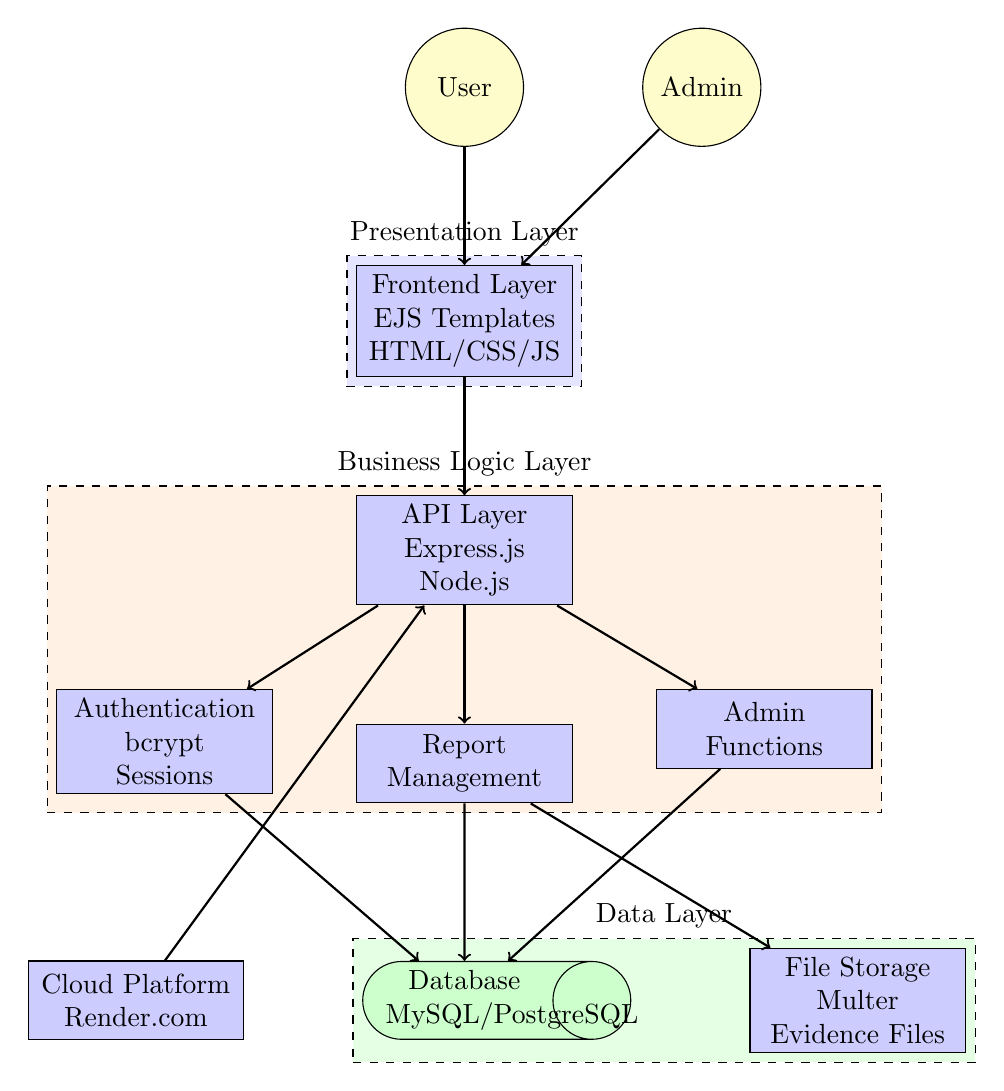
\begin{tikzpicture}[
    node distance=1.5cm,
    box/.style={rectangle, draw, fill=blue!20, text width=2.5cm, text centered, minimum height=1cm},
    database/.style={cylinder, draw, fill=green!20, text width=2cm, text centered, minimum height=1cm},
    user/.style={circle, draw, fill=yellow!20, text centered, minimum width=1.5cm},
    arrow/.style={->, thick}
]

% Users
\node[user] (user1) {User};
\node[user, right=of user1] (admin) {Admin};

% Frontend Layer
\node[box, below=of user1] (frontend) {Frontend Layer\\EJS Templates\\HTML/CSS/JS};

% API Layer
\node[box, below=of frontend] (api) {API Layer\\Express.js\\Node.js};

% Business Logic
\node[box, below left=of api] (auth) {Authentication\\bcrypt\\Sessions};
\node[box, below=of api] (reports) {Report\\Management};
\node[box, below right=of api] (admin_logic) {Admin\\Functions};

% Database Layer
\node[database, below=2cm of reports] (db) {Database\\MySQL/PostgreSQL};

% File Storage
\node[box, right=of db] (storage) {File Storage\\Multer\\Evidence Files};

% External Services
\node[box, left=of db] (cloud) {Cloud Platform\\Render.com};

% Arrows
\draw[arrow] (user1) -- (frontend);
\draw[arrow] (admin) -- (frontend);
\draw[arrow] (frontend) -- (api);
\draw[arrow] (api) -- (auth);
\draw[arrow] (api) -- (reports);
\draw[arrow] (api) -- (admin_logic);
\draw[arrow] (auth) -- (db);
\draw[arrow] (reports) -- (db);
\draw[arrow] (admin_logic) -- (db);
\draw[arrow] (reports) -- (storage);
\draw[arrow] (cloud) -- (api);

% Background boxes
\begin{scope}[on background layer]
\node[fit=(frontend), fill=blue!10, draw, dashed, label=above:Presentation Layer] {};
\node[fit=(api)(auth)(reports)(admin_logic), fill=orange!10, draw, dashed, label=above:Business Logic Layer] {};
\node[fit=(db)(storage), fill=green!10, draw, dashed, label=above:Data Layer] {};
\end{scope}

\end{tikzpicture}
\end{document}